\section{Diskussion der Umsetzung}

Petrillo et al. beschreiben in~\cite[]{PPTD08} mehrere Ursachen, die zu \textit{Feature Creep} in der Spieleentwicklung führen.
Dazu zählen unter anderem die Entwicklung eigener Lösungen anstelle der Nutzung bestehender Bibliotheken, sowie das Hinzufügen vermeintlich ``attraktiver`` Features, die unter Berücksichtigung der \textit{YAGNI}\footnote{\textit{You Aren't Gonna Need It}~\cite[]{Sch07}}-Maxime keinen Mehrwert für das eigentliche Projektziel bieten.
Damit steht die Spielentwicklung, wie die Autoren hervorheben, auf gleicher Stufe mit der ``gewöhnlichen`` Softwareentwicklung, etwa im Rahmen von Auftragsarbeiten.
Handelt es sich zudem um ein Projekt mit einer fachlich unbekannten Domäne, das in einem engen Zeitrahmen umgesetzt werden muss, sind Augenmaß und Disziplin bei der Realisierung von Funktionalität unerlässlich.
Mit helios verfolgen wir daher einen Top-Down-Ansatz, um ein schnelles Prototyping zu ermöglichen und unter Anwendung des Framework-Gedankens die schrittweise Entwicklung und Integration des \textit{Geometry Wars}-Klons voranzutreiben.
In diesem Zusammenhang verstehen wir die SOLID-Prinzipien~\cite[]{Mar03} als unverzichtbare Basis agiler Softwareentwicklung, da sie in engem Zusammenhang mit einem ``sauberen Softwaredesign`` stehen und sich im bisherigen Entwicklungsprozess bereits als wertvoll erwiesen haben\footnote{Vgl. Cabral et al., die in~\cite[]{CKME+24} SOLID im Machine-Learning-Umfeld untersuchen - einem Umfeld, das von ``iterativen Experimenten mit Daten, Modellen und Algorithmen`` (Übersetzung eigene) geprägt ist. Sie kommen zu dem Schluss, dass die Anwendung der Prinzipien wesentlich zum Quellcodeverständnis beiträgt.}.\par

Um nicht Gefahr zu laufen, am Ende der Projektphase einen \textit{Big Ball of Mud}~\cite[]{FY99} zu erzeugen, setzen wir auf eine klare Trennung der Verantwortlichkeiten, die sich in der Architektur durch die verschiedenen Feature-Layer widerspiegelt.
Über \textit{Dependency Injection}\footnote{
    Weitestgehend realisiert über Constructor Injection~\cite[]{FowlerDI}.
} wird zudem der Kopplungsgrad zwischen den beteiligten Akteuren gering gehalten~\cite[]{SZ10}.
Dies verbessert die Wartbarkeit und Testbarkeit einzelner Komponenten.\par
Da in der aktuellen Implementierung kein dedizierter DI-Container zur Anwendung kommt, entsteht durch die Verwaltung der Abhängigkeiten im eigentlichen Quelltext zusätzlicher Boilerplate-Code, der jedoch weitgehend durch die Auslagerung von Erzeugungslogik in statische Factory-Klassen reduziert wird.
Davon profitieren gerade die Implementierungen der Beispielprogramme während der Entwicklung, die auch als Testprogramme dienen.
In anderen Subsystemen unterstützen darüber hinaus Factory-Methoden die Kapselung der Objekterzeugung innerhalb jener Entitäten, denen auch fachliche Verantwortlichkeit im Sinne der Geschäftslogik zugeordnet ist~\cite[139 f.]{Eva03}.
Auf diese Weise bleibt die Architektur von helios kohärent, und Abhängigkeiten zwischen den Schichten sind auf das notwendige Minimum beschränkt.
\par

Als eher herausfordernd empfinden wir den Umgang mit modernen Sprachfeatures, die eine bewährte, aber auch ``traditionelle`` Programmiersprache wie C++ in den letzten Jahren erfahren hat - etwa das Modulsystem oder den Einsatz von Smart-Pointern: Dabei sehen wir uns im Spannungsfeld, etablierte C++-Idiome~\cite[]{IdiomaticCpp} und bewährte Konzepte in einer Entwicklungsumgebung anzuwenden, die überwiegend von Erfahrungen aus einfacheren Hochsprachen wie Java geprägt ist.
Gerade zu Beginn des Projekts wurde die Projektstruktur sowie Bezeichner von Namensräumen deshalb immer wieder angepasst (siehe Abbildung~\ref{fig:code_frequency}).\par

\begin{figure}[!h]
    \centering
    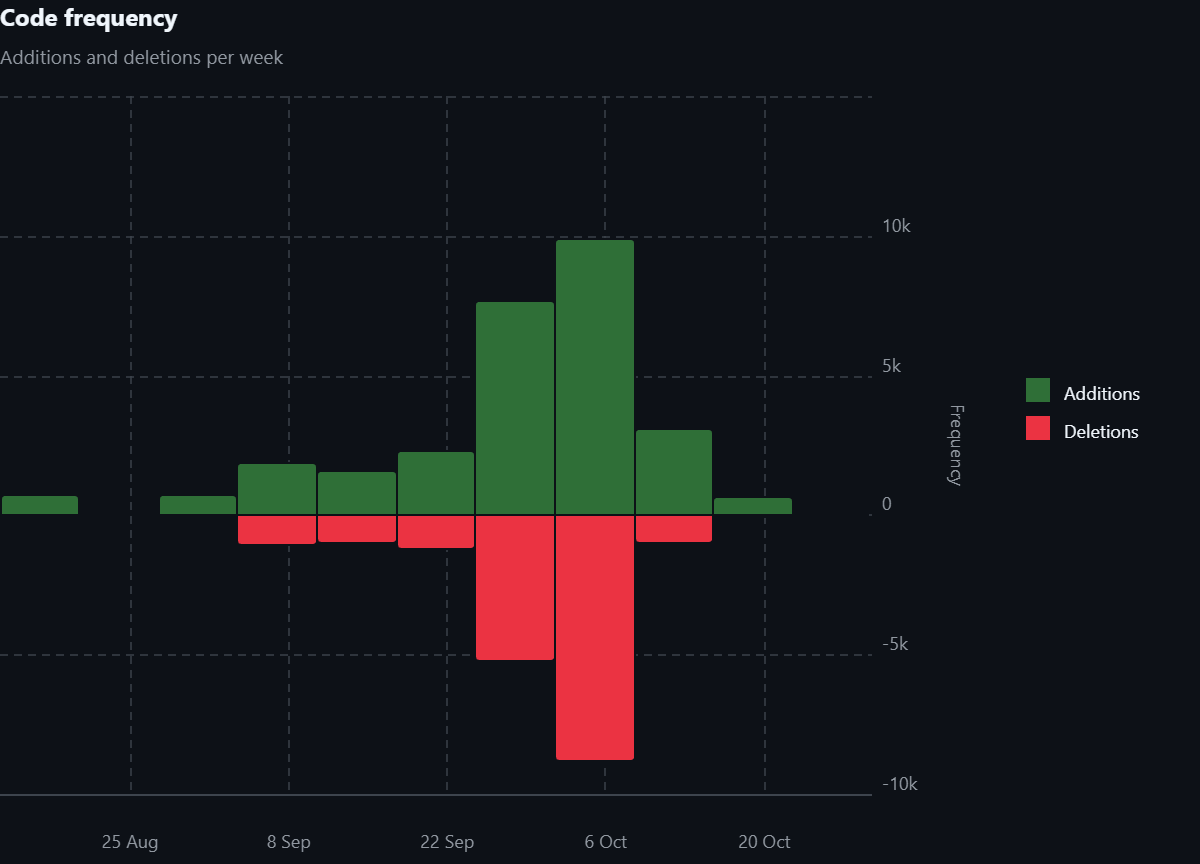
\includegraphics[width=0.8\columnwidth]{img/code_frequency}
    \caption{Code-Frequenz Graph für das helios-Repository. Die in der Frühphase erfolgten Änderungen an der Projektstruktur spiegeln sich in der nahezu symmetrischen Verteilung von hinzugefügtem (grün) und entferntem Code (rot) wider. (Quelle: GitHub)}
    \label{fig:code_frequency}
\end{figure}

Bei der Objektverwaltung über \textit{Ownership} und \textit{Pointer}-Arithmetik verzichten wir weitgehend auf \textit{raw pointer} und greifen stattdessen auf die in der Standardbibliothek definierten \texttt{unique\_ptr}, \texttt{shared\_ptr} oder \texttt{weak\_ptr}-Typen zurück, um \texttt{move}-Semantiken konsistent umzusetzen.
Inwieweit die durch den Einsatz von Smart Pointern entstehenden zusätzlichen CPU-Instruktionen - die insbesondere durch die Referenzzählung entstehen\footnote{Einen Performance-Vergleich bietet beispielsweise~\cite[]{Val25}} - beim Aufbau und der Bearbeitung der Rendering-Pipeline messbare Auswirkungen auf die Effizienz haben, muss gegebenenfalls zu einem späteren Zeitpunkt evaluiert werden.\par

Wir sehen hierin ein mögliches Optimierungspotenzial, entscheiden uns in der frühen Entwicklungsphase jedoch bewusst für Stabilität und eine klare Semantik.
Spätere  Refactorings zugunsten einer höheren Effizienz\footnote{
Diese beschränken sich nicht unbedingt auf das Design der Komponenten oder die Architektur selbst, sondern können sich bis auf niedrige Abstraktionsebenen erstrecken - etwa ``bare metal`` hin zu Implementierungen der Mathebibliothek mittels SIMD-Instruktionen, wie sie von \texttt{glm}~\cite[]{glmSimd} bereitgestellt wird (SIMD, als Abkürzung für \textit{single instruction, multiple data}, beschreibt das Konzept, bei dem eine einzelne Instruktion parallel auf unterschiedliche Daten ausgeführt wird).
} nehmen wir also in Kauf, zumal solche Maßnahmen ohnehin erst dann sinnvoll scheinen, wenn die Domäne sowohl fachlich als auch technisch hinreichend durchdrungen ist\footnote{
   Siehe ``Refactoring toward Deeper Insight``~\cite[]{Eva03}.
}.\par


Nicht unerwähnt bleiben soll an dieser Stelle die Wahl der Datenstrukturen und der Programmierparadigmen: Unsere Objektbeziehungen sind derzeit sehr ausdrucksstark (\texttt{Snapshot}, \texttt{Renderable}, \texttt{Material}, \texttt{Shader}, usw.), übermäßig tiefe Vererbungshierarchien haben wir bislang vermeiden können\footnote{
Leistungsfähige Spieleengines setzen aus Effizienzgründen häufig nicht durchgehend auf klassische OOP-Paradigmen, sondern verwenden in performance-kritischen Subsystemen einen datenorientierten Ansatz, bei dem flache Verbünde von Komponenten nach dem \textit{ECS Pattern}~\cite[]{RCCK25} deutliche Performancevorteile aufweisen können~\cite[]{WWM22}.
}.
Die Entscheidung, Vektoren als primäre Datencontainer zu verwenden, kann sich potenziell negativ auf die Rendering-Pipeline auswirken, wenn die Render-Queue nach einer Aktualisierung der Szene neu aufgebaut und dabei zusätzlicher Speicher zur Laufzeit alloziiert werden muss.\par

Weitere Optimierungspotenziale sehen wir im Design des \texttt{EventManagers} und der Eingabeverarbeitung: Beide Systeme können zusammengeführt werden, sodass auch Eingabebefehle nach dem Prinzip ``Don't call us, we call you`` als Ereignisse an interessierte Beobachter weitergeleitet werden.
Dabei ist zu berücksichtigen, dass entsprechende Schnittstellen dem Spiel zur Verfügung gestellt werden müssen und eine Bottom-up Kommunikation erlaubt sein muss~\cite[]{BMRS+96}.
Darüber hinaus soll eine Mechanik geschaffen werden, welche aus den Eingabeereignissen entsprechende \texttt{ControlCommand}s erzeugen, die vom Spiel als eigentliche  Steuerparameter interpretiert werden~\cite[21 ff.]{Nys14}.\par

Bei der Architektur des Rendering-Systems sehen wir eine Grundlage für eine modulare und erweiterbare Rendering-Pipeline, die derzeit eine klare Trennung zwischen Szenenbeschreibung und eigentlichem Rendering realisiert.
Der Vorteil des gewählten Designs liegt darin, dass die individuellen \texttt{RenderPass}-Instanzen mit zusätzlichen Optionen konfiguriert werden können (bspw. \textit{Depth Testing}, \textit{Draw Mode}, \textit{Anti-Aliasing} u.a.) und die \texttt{RenderQueue}s so sortiert werden können, dass die Kommunikation mit der GPU möglichst effizient stattfinden kann\footnote{
    Unity~\cite[]{UnityRenderQueue} und OGRE~\cite[]{OgreRenderQueue} verfolgen ähnliche Konzepte; auch Diskussionen von Christer Ericson~\cite[]{ChristerEricson} thematisieren die Sortierung des Render-Pass. Vulkan bietet explizite Render-Pass-Semantik~\cite[]{VulkanRenderPass}
}.
Ob sich das Design im Rahmen der Implementierung des eigentlichen Spiels bewährt - und diese Features überhaupt benötigt werden - wird sich in der weiteren Entwicklung zeigen.



